% Base template source: https://tex.stackexchange.com/questions/8827/preparing-cheat-sheets

\documentclass[10pt,landscape]{article}

\usepackage{multicol}
\usepackage{lipsum}

\usepackage{calc, ifthen,hyperref, gensymb, comment, textcomp}

\usepackage{amsmath,amsthm,amsfonts,amssymb}

\usepackage{color,graphicx,overpic}

\usepackage{geometry}
% This sets page margins to .5 inch if using letter paper, and to 1cm
% if using A4 paper. (This probably isn't strictly necessary.)
% If using another size paper, use default 1cm margins.
\ifthenelse{\lengthtest { \paperwidth = 11in}}
    { \geometry{top=.25in,left=.25in,right=.25in,bottom=.25in} }
    {\ifthenelse{ \lengthtest{ \paperwidth = 297mm}}
        {\geometry{top=1cm,left=1cm,right=1cm,bottom=1cm} }
        {\geometry{top=1cm,left=1cm,right=1cm,bottom=1cm} }
    }

% Turn off header and footer
\pagestyle{empty}

% Don't print section numbers
\setcounter{secnumdepth}{0}

% Define Image
\newenvironment{Figure}
     {\par\medskip\noindent\minipage{\linewidth}}
     {\endminipage\par\medskip}
    
% Define Line Spacing
\linespread{.3}
% -----------------------------------------------------------------------

\begin{document}
\raggedright
\footnotesize

% Area Above Columns
\begin{center}
     \Large{\underline{Thermodynamics - Zak Olech - \today}}
\end{center}
\begin{multicols}{3}

% multicol parameters
% These lengths are set only within the two main columns
\setlength{\columnseprule}{0.25pt}
\setlength{\premulticols}{1pt}
\setlength{\postmulticols}{1pt}
\setlength{\multicolsep}{1pt}
\setlength{\columnsep}{2pt}

\begin{comment}
\section{Variables (Alphbetical By Variable)}
\begin{equation}
    A=\text{area}
\end{equation}
\begin{equation}
    \chi=\text{exergy}
\end{equation}
\begin{equation}
    E=\text{energy}=U+KE+PE
\end{equation}
\begin{equation}
    h=\text{enthalpy}
\end{equation}
\begin{equation}
    k=\text{Vapor-Liquid Equilibrium Point}
\end{equation}
\begin{equation}
    m = \text{mass}
\end{equation}
\begin{equation}
    \dot{m}=\rho*\dot{V}=\text{mass flow rate}
\end{equation}
\begin{equation}
    P=\text{pressure}
\end{equation}
\begin{equation}
    q= \text{heat}
\end{equation}
\begin{equation}
    \rho = \frac{m}{v}= \text{density}
\end{equation}
\begin{equation}
    S= \text{entropy}
\end{equation}
\begin{equation}
    T= \text{temperature}
\end{equation}
\begin{equation}
    u= \text{internal energy}
\end{equation}
\begin{equation}
    V= \text{volume}
\end{equation}
\begin{equation}
    \vec{V}= \text{velocity}
\end{equation}
\begin{equation}
    \vee = \frac{V}{m}=\frac{1}{\rho}= \text{specific volume}
\end{equation}
\begin{equation}
    W=\text{work}
\end{equation}
\begin{equation}
    x= \text{quality}
\end{equation}
\begin{equation}
    z=\text{height from an axis}
\end{equation}
\end{comment}

% -----------------------------------------------------------------------
\section{General Information}
\subsection{Conversion Factors}
1 pascal        = 1 $\frac{\text{newton}}{\text{meter}^2}$\\*
1 kilopascal    = $10^3$ pa\\*
1 megapascal    = $10^6$ pa\\*
1 gigapascal    = $10^9$ pa\\*
\subsection{Process}
1 - Assumptions\\*
2 - Properties\\*
3 - Analysis\\*
\subsection{Assumptions}
- Typically Air is assumed to be an Ideal Gas\\*
- Room Temperature = 300 k

\section{Physically Meaningful Formulas}
\subsection{Mass Balance}
\begin{equation}
    m_{in}-m_{out}=\Delta m_{system}
\end{equation}
\subsection{Energy Balance}
\begin{equation}
    E_{in}-E_{out}=\Delta E_{system}
\end{equation}
\subsection{Entropy Balance}
\begin{equation}
    S_{in}-S_{out}+S_{gen}=\Delta S_{system}
\end{equation}
\subsection{Exergy Balance}
\begin{equation}
    X_{in}-X_{out}=X_{destroyed}=\Delta X_{system}
\end{equation}

\section{Chapter 1 - Introduction and Basic Concepts}
%\subsection{1-2 Thermodynamics and Energy}
\subsection{1-3 Importance of Dimensions and Units}
\begin{equation}
    T(K)=T(\degree C)+273.15
\end{equation}
\begin{equation}
    \Delta T(K)=\Delta T(\degree C)
\end{equation}
\begin{equation}
    T(R)=T(\degree F)+459.67
\end{equation}
\begin{equation}
    \Delta T(R)=\Delta T(\degree F)
\end{equation}
%\subsection{1-4 Properties of a System}
%\subsection{1-5 Density and Specific Gravity}
%\subsection{1-6 State and Equilibrium}
%\subsection{1-7 Processes and Cycles}
%\subsection{1-8 Temperature and the Zeroth Law of Thermodynamics}
\subsection{1-9 Pressure}
\begin{equation}
    P_{gage}=P_{abs}-P_{atm}
\end{equation}
\begin{equation}
    P_{vac}=P_{atm}-P_{abs}
\end{equation}
\begin{equation}
    P=P_{atm}+\rho gh
\end{equation}
\begin{equation}
    P_{gage}=\rho gh
\end{equation}
%\subsection{1-10 Pressure Measurement Devices}
%\subsection{1-11 Problem-Solving Technique}

\section{Chapter 2 - Energy, Energy Transfer, and General Energy Analysis}
%\subsection{2-1 Introduction}
\subsection{2-2 Forms of Energy}
\begin{equation}
    KE=m\frac{V^2}{2}
\end{equation}
\begin{equation}
    PE=mgz
\end{equation}
\begin{equation}
    E=U+KE+PE=U+m\frac{V^2}{2}+mgz
\end{equation}
\begin{equation}
    \dot{m}=\rho\dot{\vee}=\rho A_cV_{avg}
\end{equation}
\begin{equation}
    \dot{E}=\dot{m}e
\end{equation}
\begin{equation}
    \dot{E}_{mech}=\dot{m}e_{mech}=\dot{m}(\frac{P}{\rho}+\frac{V^2}{2}+gz)
\end{equation}
\subsection{2-3 Energy Transfer by Heat}
\begin{equation}
    Q=\int^{t_2}_{t_1}\dot{Q}dt
\end{equation}
\begin{equation}
    Q=h_2-h_1
\end{equation}
%\subsection{2-4 Energy Transfer by Work}
%\subsection{2-5 Mechanical Forms of Work}
\subsection{2-6 First Law of Thermodynamics}
\begin{equation}
    \Delta E_{system}=E_{final}-E_{initial}=\Delta E=\Delta U + \Delta KE + \Delta PE
\end{equation}
\begin{equation}
    \Delta U = m(u_2-u_1)
\end{equation}
\begin{equation}
    \Delta KE=\frac{1}{2}m(V_2^2-V_1^2)
\end{equation}
\begin{equation}
    \Delta PE=mg(z_2-z_1)
\end{equation}
\begin{equation}
    \begin{aligned}
        \dot{Q}_{net}-\dot{W}_{net}+\Sigma\dot{m}_{in}(h+\frac{\vec{V}^2}{2}+gz)_{in}\\
        -\Sigma\dot{m}_{out}(h+\frac{\vec{V}^2}{2}+gz)_{out}=\Delta\dot{E}_{sys}
    \end{aligned}
\end{equation}
%\subsection{2-7 Energy Conversion Efficiencies}

\section{Chapter 3 - Properties of Pure Substances}
%\subsection{3-1 Pure Substances}
%\subsection{3-2 Phases of a Pure Substances}
%\subsection{3-3 Phase-change Processes of Pure Substances}
%\subsection{3-4 Property Diagrams for Phase-change Processes}
\subsection{3-5 Property Tables}
\subsubsection{Quality}
\begin{equation}
    x=\frac{m_{vapor}}{m_{total}}
\end{equation}
\begin{equation}
    y=y_f+x*y_{fg}
\end{equation}
\begin{equation}
    y_{fg}=y_g-y_f
\end{equation}
\subsection{3-6 Ideal-Gas Equation of State}
\begin{equation}
    P\vee=RT
\end{equation}
\begin{equation}
    P\vee=RT
\end{equation}
\begin{equation}
    R=\frac{R_u}{m}
\end{equation}
\begin{equation}
    P\vee=ZRT
\end{equation}
\begin{equation}
    \frac{P_2V_2}{T_2}\frac{P_1V_1}{T_1}
\end{equation}
\begin{equation}
    V_1=\frac{RT_1}{P_1}
\end{equation}

\section{Chapter 4 - Energy Analysis of a Closed System}
\subsection{4-1 Moving Boundary Work}
\subsubsection{General}
\begin{equation}
    W_b=\int^2_1Pd\vee
\end{equation}
\subsubsection{Isobaric process (P1=P2)}
\begin{equation}
    W_b=P_0(\vee_2-\vee_1)
\end{equation}
\subsubsection{Isothermal Process of an Ideal Gas}
\begin{equation}
    W_b=P_1\vee_1ln\frac{\vee_2}{\vee_1}=mRT_0ln\frac{\vee_2}{\vee_1}
\end{equation}
\subsection{4-2 Energy Balance for Closed Systems}
\begin{equation}
    Q_{net}-W_{net}=\Delta U + \Delta KE + \Delta PE
\end{equation}
\begin{equation}
    W=W_{other}+W_b
\end{equation}
\begin{equation}
    \Delta U = m(u_2-u_1)
\end{equation}
\begin{equation}
    \Delta KE = \frac{1}{2}m(V^2_2-V_1^2)
\end{equation}
\begin{equation}
    \Delta PE = mg(z_2-z_1)
\end{equation}
\subsubsection{Constant-Pressure Process}
\begin{equation}
    Q-W_{other}=\Delta H+\Delta KE + \Delta PE
\end{equation}
\subsection{4-3 Specific Heats}
\begin{equation}
    c_{constant volume}=(\frac{\delta u}{\delta T})
\end{equation}
\begin{equation}
    c_{constant pressure}=(\frac{\delta h}{\delta T})
\end{equation}
\subsection{4-4 Internal Energy, Enthalpy, and Specific Heats of Ideal Gases}
\begin{equation}
    \Delta u=u_2-u_1=\int^2_1c_v(T)dT=c_{v,avg}(T_2-T_1)
\end{equation}
\begin{equation}
    \Delta h=h_2-h_1=\int^2_1c_p(T)dT=c_{p,avg}(T_2-T_1)
\end{equation}
\begin{equation}
    c_p=c_v+R
\end{equation}
\begin{equation}
    k=\frac{c_p}{c_v}
\end{equation}
\subsection{4-5 Internal Energy, Enthalpy, and Specific Heats of Solids and Liquids}
\subsubsection{Incompressible Substances}
\begin{equation}
    c_p=c_v=c
\end{equation}
\begin{equation}
    \Delta u=\int^2_1c(T)dt=c_{avg}(T_2-T_1)
\end{equation}
\begin{equation}
     \Delta h = \Delta u + \vee\Delta P
\end{equation}
\subsubsection{CV and CP Relationships}
\begin{equation}
    C_V=\frac{\delta u}{\delta T}_V=(\frac{du}{dT})_{I.G}
\end{equation}
\begin{equation}
    C_P=(\frac{\delta h}{\delta T})_P=(\frac{dh}{dT})_{I.G}
\end{equation}

\section{Chatper 5 - Mass and Energy analysis of Control Volumes}
\subsection{5-1 Conservation of Mass}
\begin{equation}
    m_{in}-m_{out}=m_{system}
\end{equation}
\begin{equation}
    \dot{m}=\rho VA
\end{equation}
\subsection{5-2 Flow Work and the energy of a Flowing Fluid}
\subsubsection{Total Energy of a Flowing Fluid}
\begin{equation}
    \theta=h+ke+pe=h+\frac{V^2}{2}+gz
\end{equation}
\subsubsection{Energy Transport by Mass}
\begin{equation}
    E_{mass}=m*\theta=m(h+\frac{V^2}{2}+gz)
\end{equation}
\subsection{5-3 Energy Analysis of Steady-Flow Systems}
\begin{equation}
    \Sigma_{in}\dot{m}=\Sigma_{out}\dot{m}
\end{equation}
\begin{equation}
    \dot{Q}-\dot{W}=\Sigma_{out}\dot{m}(h+\frac{V^2}{2}+gz)-\Sigma_{in}\dot{m}(h+\frac{V^2}{2}+gz)
\end{equation}
%\subsection{5-4 Some Steady-Flow Engineering Devices}
\subsection{5-5 Energy Analysis of Unsteady-Flow Processes}
\begin{equation}
    m_{in}-m_{out}=\Delta m_{system}
\end{equation}
\begin{equation}
    \begin{split}
        (Q_{in}-Q_{out})-(W_{out}-W_{in})\\
        =\Sigma_{out}mh-\Sigma_{in}mh+(m_2u_2-m_1u_1)_{system}
    \end{split}
\end{equation}

\section{Chapter 6 - The Second Law of Thermodynamics}
Kelvin-Plank Statement, Clausius Statement
\subsection{6-1 Intro to Second Law}
\subsection{6-2 Thermal Energy Reservoirs}
\subsection{6-3 Heat Engines}
\begin{equation}
    Thermal efficiency = \frac{Net work output}{Total heat input}
\end{equation}
\begin{equation}
    \eta_{th}=\frac{W_{net,out}}{Q_{in}}=1-\frac{Q_{out}}{Q_{in}}
\end{equation}
\subsection{6-4 Refrigerators and Heat Pumps}
\subsubsection{Coefficient of Performance}
\begin{equation}
    \text{COP}=\frac{\text{desired result}}{\text{required input}}
\end{equation}
\begin{equation}
     COP_{refrigerator}=\frac{Q_L}{Q_H-Q_L}=\frac{1}{Q_H/Q_L-1}
\end{equation}
\begin{equation}
    COP_{HP}=\frac{desired output}{required input}=\frac{Q_h}{w_{net,in}}
\end{equation}
\begin{equation}
    COP_{HP}=\frac{Q_H}{Q_H-Q_L}=\frac{1}{1-Q_L/Q_H}
\end{equation}
\begin{equation}
    COP_{HP}=COP_R+1
\end{equation}
\subsection{6-5 Perpetual-Motion Machines (PPM LN)}
%\subsection{6-6 Reversible and Irreversible Processes}
\subsection{6-7 The Carnot Cycle}
\subsection{6-8 The Carnot Principles}
\subsection{6-9 The Thermodynamic Temperature Scale}
\begin{equation}
    (\frac{Q_H}{Q_L})_{rev}=\frac{T_H}{T_L}
\end{equation}
\subsection{6-10 The Carnot Heat Engine}
\begin{equation}
    \chi_{th,rev}=1-\frac{T_L}{T_H}
\end{equation}
\subsection{6-11 the Carnot Refrigerator and Heat Pump}
\begin{equation}
    COP_{R,rev}=\frac{1}{T_h/T_L-1}
\end{equation}
\begin{equation}
    COP_{HP,rev}=\frac{1}{1-T_L/T_H}
\end{equation}

\section{Chapter 7 - Entropy}
\subsection{7-1 Entropy}
\begin{equation}
    dS=(\frac{dQ}{T})_{int,rev}
\end{equation}
\subsubsection{Internally reversible, isothermal process}
\begin{equation}
    \Delta S = \frac{Q}{T_0}
\end{equation}
\subsection{7-2 The Increase of Entropy Principle}
\begin{equation}
\S_{gen}\geq0    
\end{equation}
\subsubsection{Entropy Generation}
\begin{equation}
    S_{heat}=\frac{q}{T}
\end{equation}
\begin{equation}
    S_{mass}=mS
\end{equation}
\subsection{7-3 Entropy Change}
\begin{equation}
    \Delta S = S_1-S_2
\end{equation}
\subsubsection{Pure Substance}
\subsubsection{PS - Any Process}
\begin{equation}
    \Delta S_2-S_1
\end{equation}
\subsubsection{PS - Isentropic Process}
\begin{equation}
    S_2=S_1
\end{equation}
\subsubsection{Incompressible Substance}
\subsubsection{IS - Any Process}
\begin{equation}
    S_2-S_1=c_{avg}ln\frac{T_2}{T_1}
\end{equation}
\subsubsection{IS - Isentropic Process}
\begin{equation}
    T_2=T_1
\end{equation}
\subsubsection{Ideal Gases}
\subsubsection{IG - Constant Specific Heats}
\subsubsection{IG - CSH - Any Process}
\begin{equation}
    \Delta S = C_{v,avg}ln(\frac{T_2}{T_1})+Rln(\frac{V_2}{V_1})
\end{equation}
\begin{equation}
    \Delta S = C_{p,avg}ln(\frac{T_2}{T_1})-Rln(\frac{P_2}{P_1})
\end{equation}
\subsubsection{IG - CSH - Isentropic Process}
\begin{equation}
   (\frac{T_2}{T_1})_{s=const}=(\frac{\vee_1}{\vee_2})^{k-1} 
\end{equation}
\begin{equation}
    (\frac{T_2}{T_1})_{s=const}=(\frac{P_2}{P_1})^{(k-1)/k}
\end{equation}
\begin{equation}
    (\frac{P_2}{P_1})_{s=const}=(\frac{\vee_1}{\vee_2})^k
\end{equation}
\subsubsection{IG - Variable Specific Heats}
\subsubsection{IG - VSH - Any Process}
\begin{equation}
    \Delta S = S_2^{\degree} - S_1^{\degree} - Rln(\frac{P_2}{P_1})
\end{equation}
\subsubsection{IG - VSH - Isentropic Process}
\begin{equation}
    S^\degree_2=S_1^\degree+Rln\frac{P_2}{P_1}
\end{equation}
%\subsection{7-4 Isentropic Processes}
%\subsection{7-5 Property Diagrams Involving Entropy}
%\subsection{7-6 What is Entropy?}
\subsection{7-7 The T ds Relations}
\begin{equation}
    Tds=du+Pdv
\end{equation}
\begin{equation}
    Tds=dh-vdP
\end{equation}
%\subsection{7-8 Entropy Change of Liquids and Solids}
%\subsection{7-9 The Entropy Change of Ideal Gases}
%\subsection{7-10 Reversible Steady-Flow Work}
%\subsection{7-11 Minimizing the Compressor Work}
\subsection{7-12 Isentropic Efficiencies of Steady-Flow Devices}
\begin{equation}
    \chi_T=\frac{Actual turbine work}{Isentropic turbine work}=\frac{w_a}{w_s}=\frac{h_1-h_{2a}}{h_1-h_{2s}}
\end{equation}
\begin{equation}
    \chi_T=\frac{Isentropic Compressor Work}{Actual Compressor Work}=\frac{w_s}{w_a}=\frac{h_{2s}-h_1}{h_{2a}-h_1}
\end{equation}
\begin{equation}
    \chi_T=\frac{Actual KE at nozzle exit}{Isentropic KE At Nozzle Exit}=\frac{V^2_{2a}}{V^2_{2s}}=\frac{h_1-h_{2a}}{h_1-h_{2s}}
\end{equation}
\subsection{7-13 Entropy Balance}
\begin{equation}
    S_{in}-S_{out}+S_{gen}=\Delta S_{system}
\end{equation}
\subsubsection{Steady-Flow}
\begin{equation}
    S_{gen}=\Sigma \dot{m_e}S_e-\Sigma\dot{m_i}-\Sigma\frac{\dot{Q_K}}{T_k}
\end{equation}
\subsubsection{Steady-Flow Work}
\begin{equation}
    w_{rev}=-\int^2_1\vee dP-\Delta ke - \Delta pe
\end{equation}
\section{General}
\begin{equation}
    \text{x does not equal quality --- }\int\frac{1}{x}dxln(\frac{x_2}{x_1})
\end{equation}
\begin{equation}
    h=u+P*V
\end{equation}
\begin{equation}
    (\frac{T_2}{T_1})=(\frac{v_1}{v_2})^{k-1}=(\frac{P_2}{P_1})^{\frac{k-1}{k}}
\end{equation}

\begin{comment}
\subsection{Chapter 8 - Exergy}
\subsubsection{Exergy Balance}
\begin{equation}
    \chi_{in}-\chi_{out}-\chi_{dest}=\Delta x
\end{equation}
\begin{equation}
    \chi_{\text{heat}}=(1-\frac{T_c}{T})q
\end{equation}
\subsubsection{Exergy Change - Closed System}
\begin{equation}
    \begin{aligned}
        \Delta\chi=\Delta\phi=(u_2-u_1)+P_0(\vee_2-\vee_1)-T_0(S_2-S_1) \\
        +\frac{\vec{V}_2^2-\vec{V}_1^2}{2}+g(z_2-z_1)
    \end{aligned}
\end{equation}
\subsubsection{Exergy Change - Control Volume}
\begin{equation}
    W_{flow}=P*\vee
\end{equation}
\begin{equation}
    \chi_{\text{flow,stream}}=(h-h_0)-T_0(S-S_0)+\frac{\vec{V}^2}{2}+gz
\end{equation}
\begin{equation}
    \Delta\chi=\chi_2-\chi_1
\end{equation}
\subsubsection{Exergy Balance - Closed System}
\begin{equation}
    \chi=(u-u_0)+P_0(\vee-\vee_0)-T_0(S-S_0)+\frac{\vec{V}^2}{2}+gz
\end{equation}
\subsubsection{Exergy Balance - Control Volume}
\begin{equation}
    \chi=(h-h_0)-T_0(S-S_0)+\frac{\vec{V}^2}{2}+gz
\end{equation}
\end{comment}


\section{Chapter 9}
\subsection{Air-Standard Otto cycle}
\begin{Figure}
    \centering
    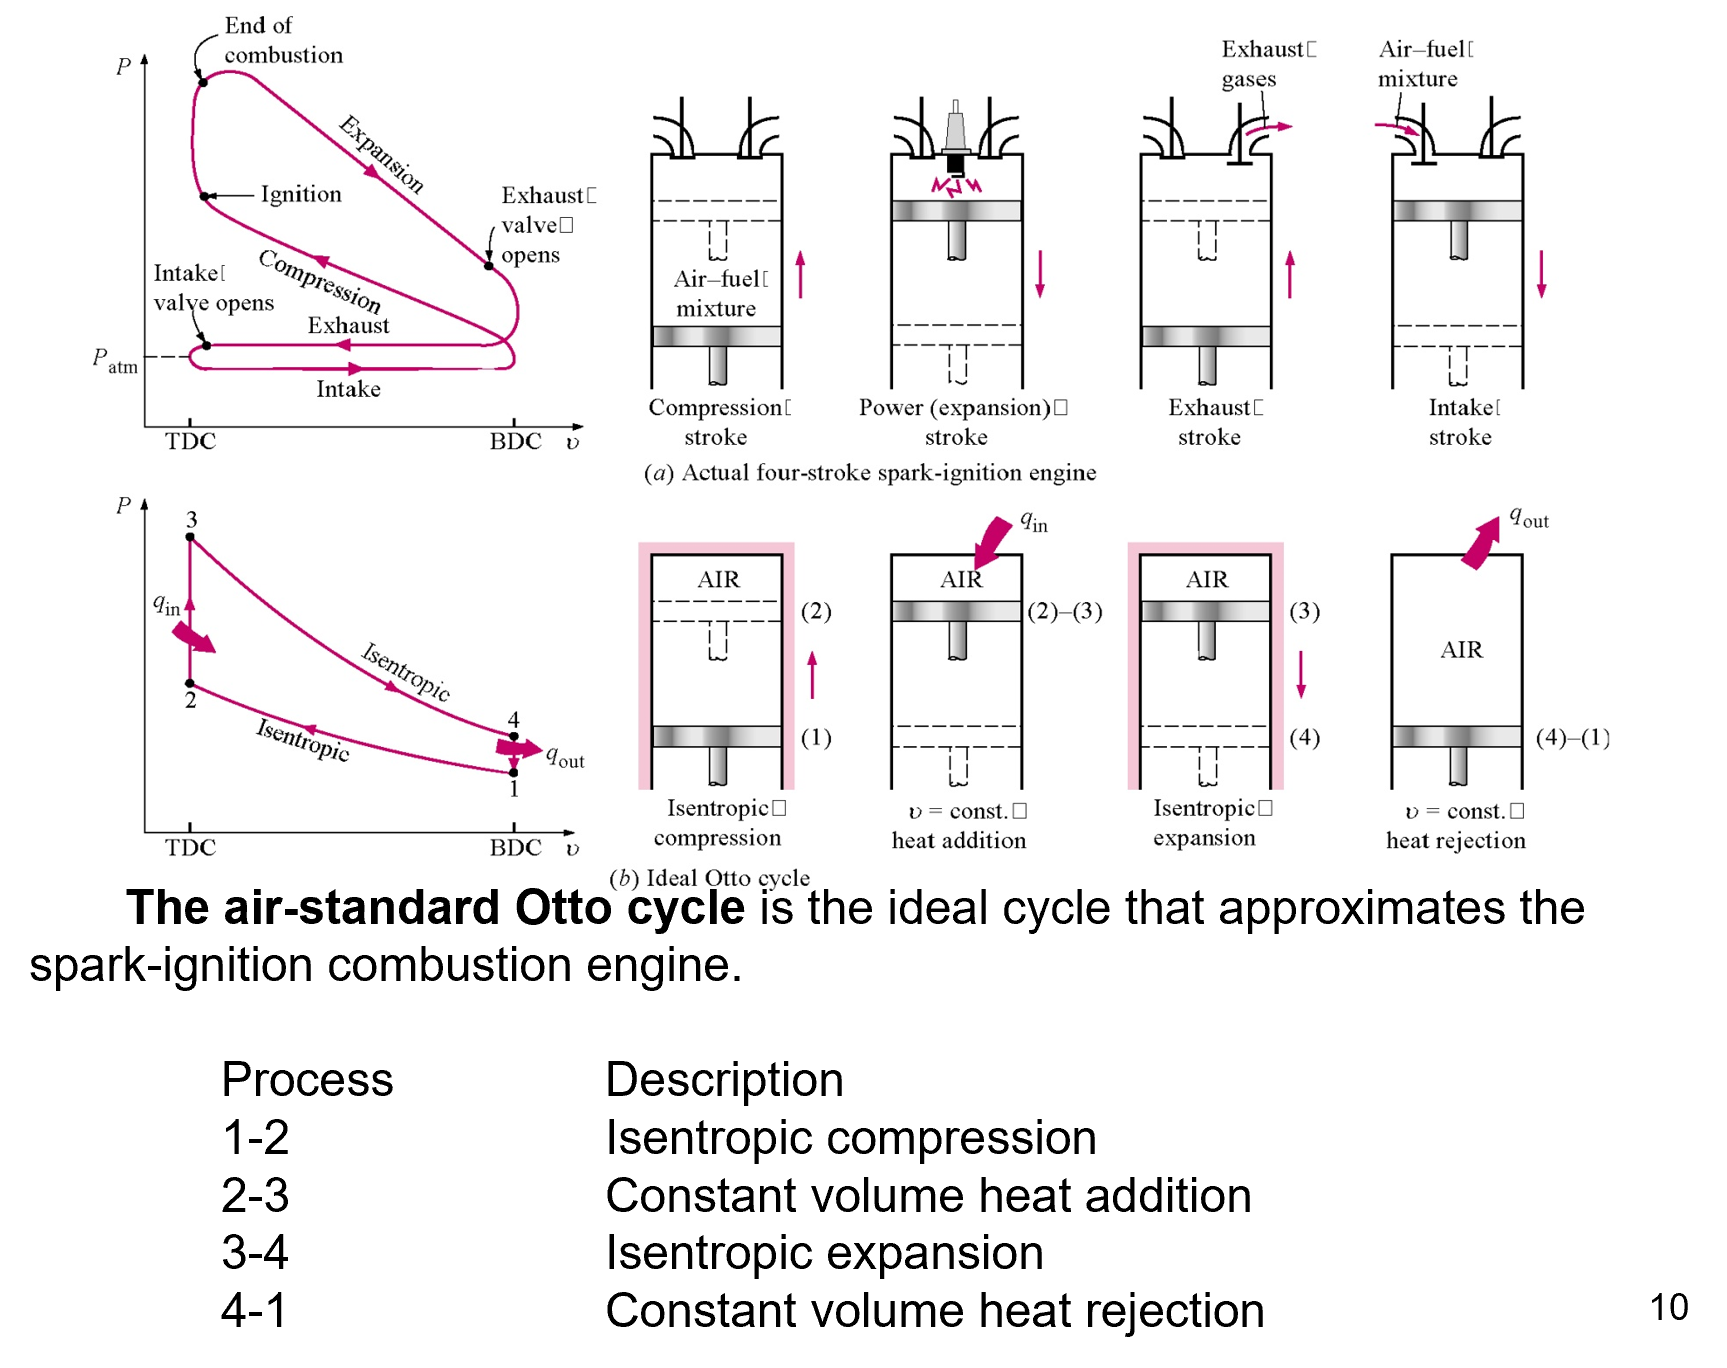
\includegraphics[width=\linewidth, height=5cm]{Air-Standard_OttoCycle.png}
\end{Figure}
\begin{Figure}
    \centering
    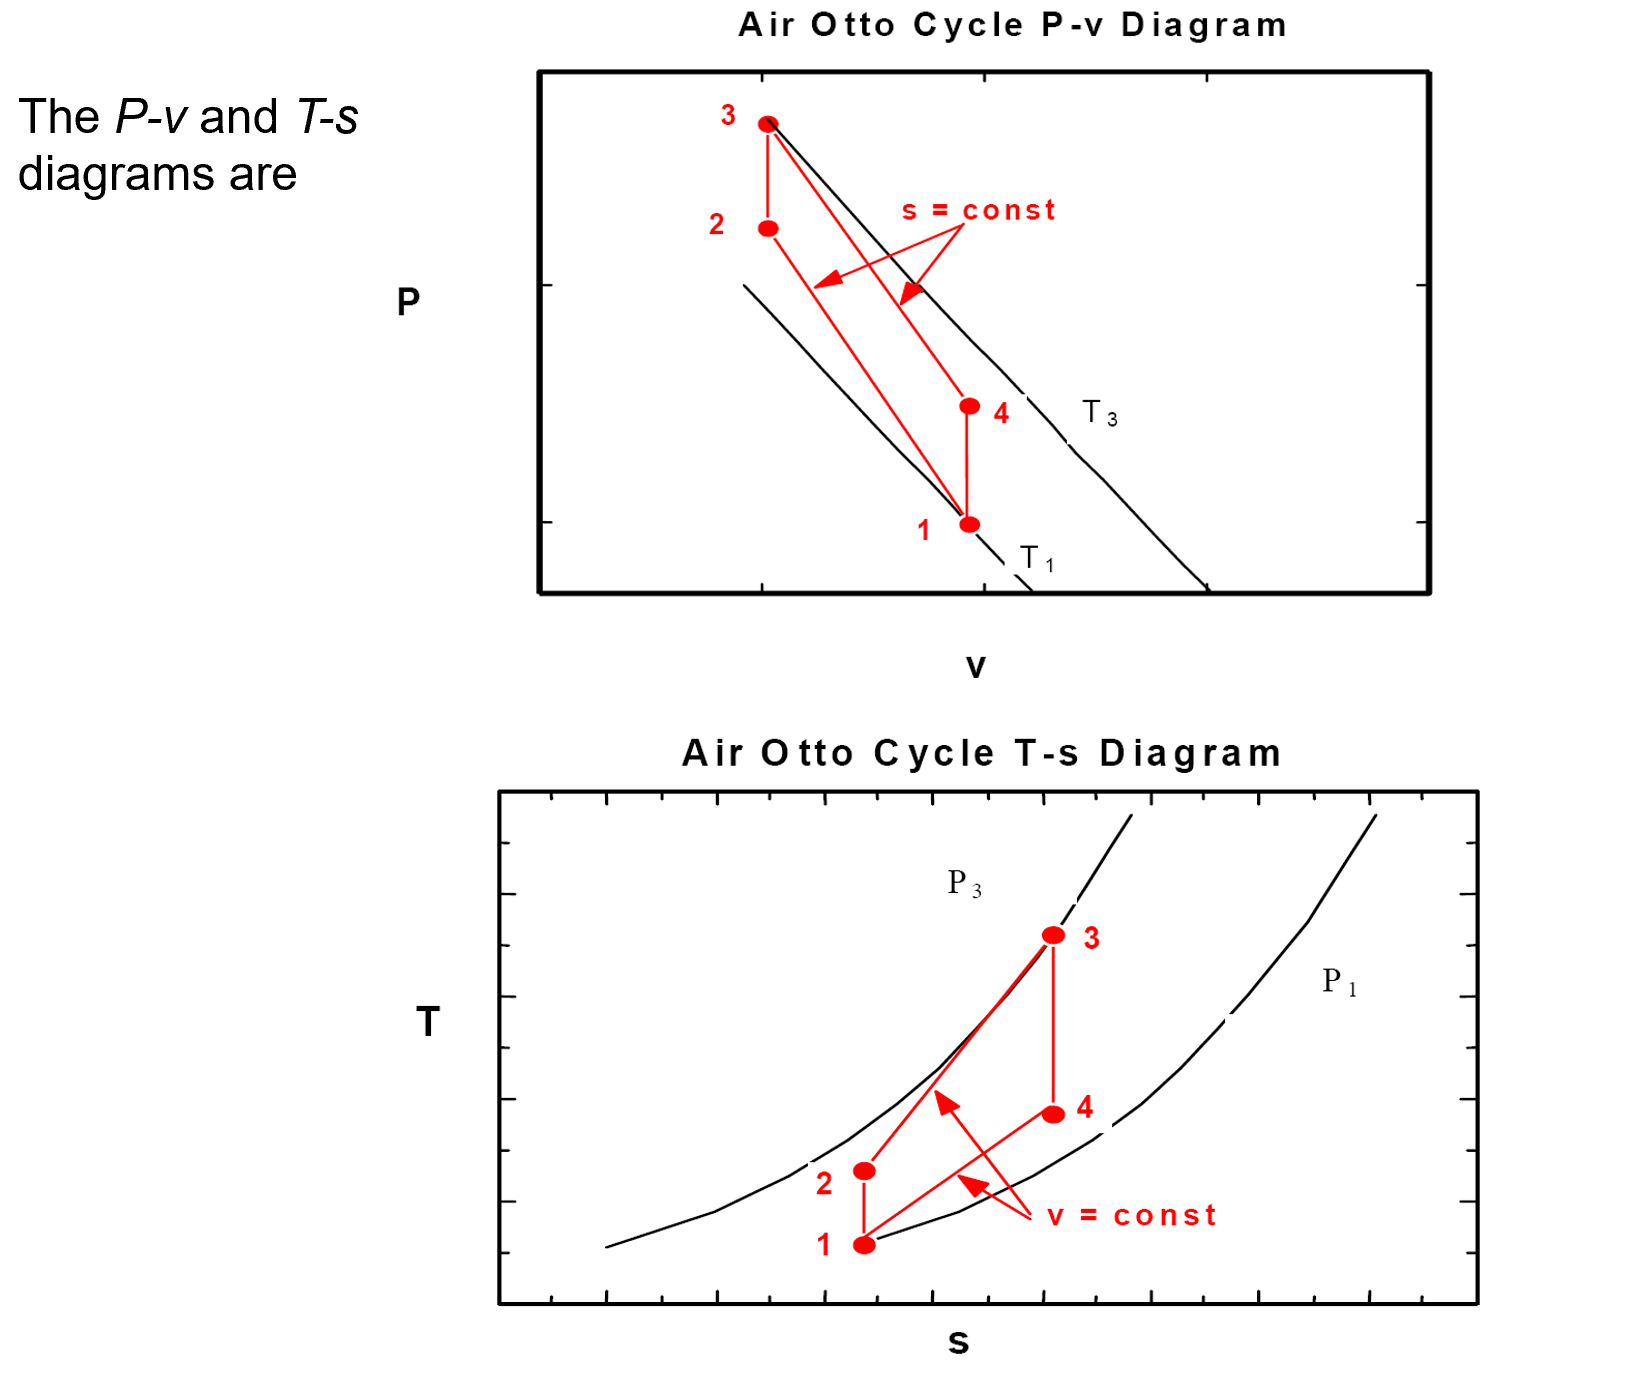
\includegraphics[width=\linewidth, height=5cm]{Air-Standard_OttoCycle_PVTS.png}
\end{Figure}
\subsubsection{Compressoin Ratio}
\begin{equation}
    r=\frac{Vmax}{Vmin}=\frac{V_{BDC}}{V_{TDC}}
\end{equation}
\subsubsection{Mean Effective Pressure (MEP)}
\begin{equation}
    \text{MEP}=\frac{W_{net}}{V_{max}-V_{min}}
\end{equation}
\subsubsection{Thermal Efficiency}
\begin{equation}
    \eta_{th,Otto}=1-\frac{Q_{out}}{Q_{in}}=1-\frac{mC_v(T_4-T_1)}{mC_v(T_3-T_2)}
\end{equation}
\subsubsection{Back Work Ratio}
\begin{equation}
    BWR=\frac{W_{comp}}{W_{exp}}=\frac{\delta u_{12}}{-\delta u_{34}}=\frac{C_v()T_2-T_1}{C_v(T_3-T_4)}=\frac{T_2-T_1}{T_3-T_4}
\end{equation}

\subsection{Air-Standard Diesel Cycle}
\begin{Figure}
    \centering
    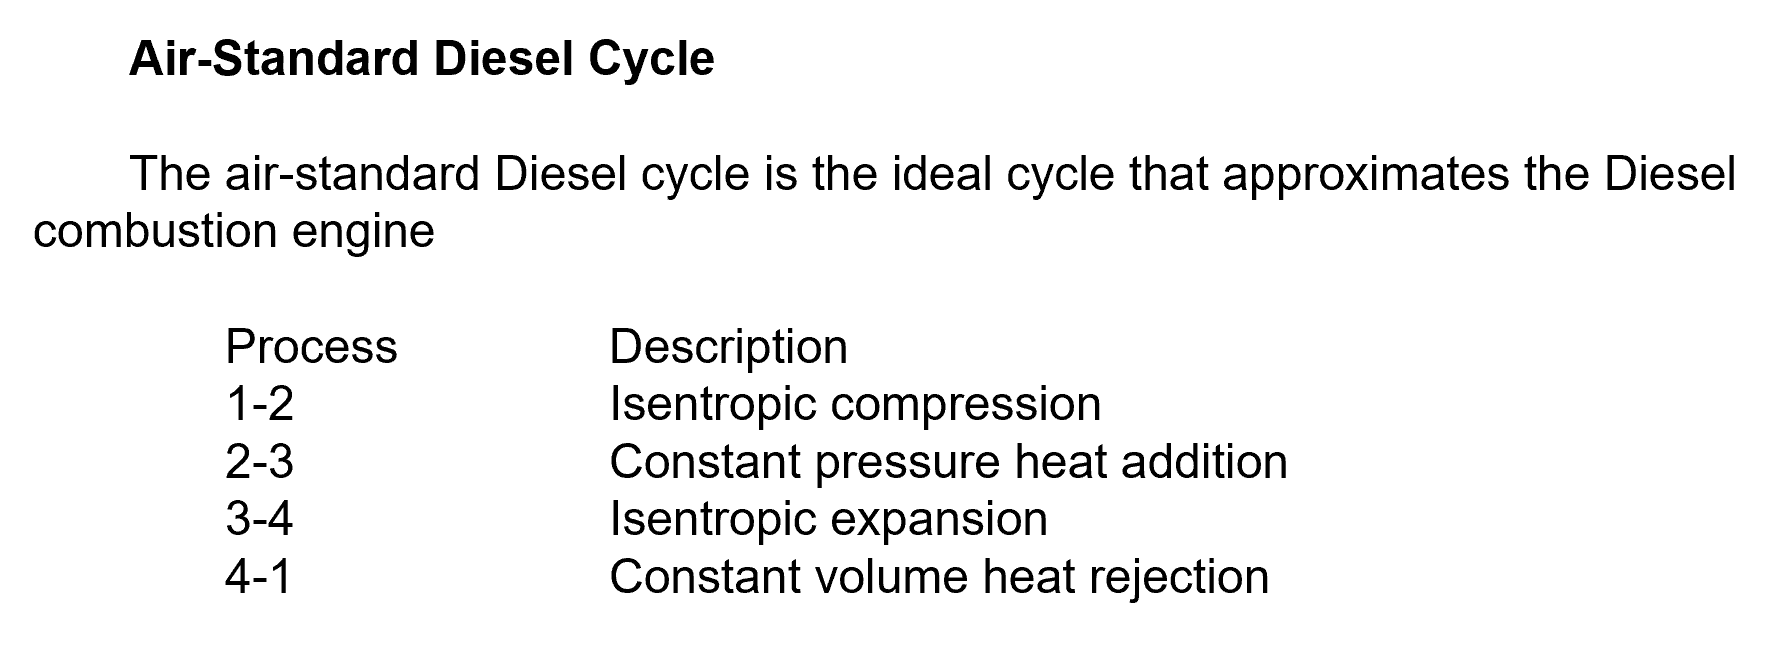
\includegraphics[width=\linewidth, height=5cm]{Air-Standard_DieselCycle.png}
\end{Figure}
\begin{Figure}
    \centering
    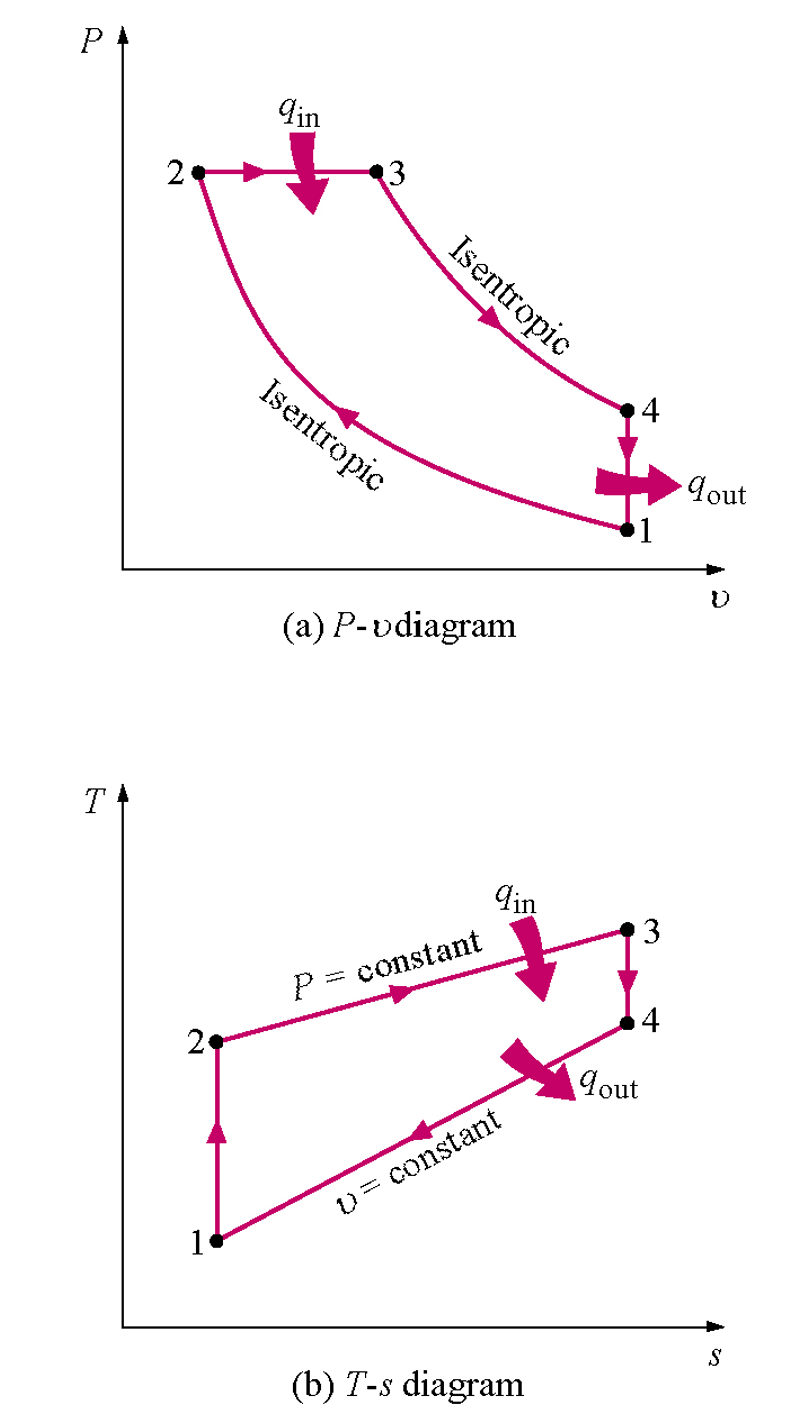
\includegraphics[width=\linewidth, height=5cm]{Air-Standard_DieselCycle_PVTS.png}
\end{Figure}
\subsubsection{Thermal Efficiency}
\begin{equation}
    \begin{split}
        \eta_{th,Diesel}=1-\frac{Q_{out}}{Q_{in}}=1-\frac{mC_v(T_4-T_1)}{mC_p(T_3-T_2)}\\
        =1-\frac{1}{k}\frac{T_1(T_4/T_1-1)}{T_2(T_3/T_2-1)}=1-\frac{1}{r^{k-1}}\frac{r^l_c-1}{k(r_c-1)}
    \end{split}
\end{equation}

\subsection{Brayton Cycle}
\begin{Figure}
    \centering
    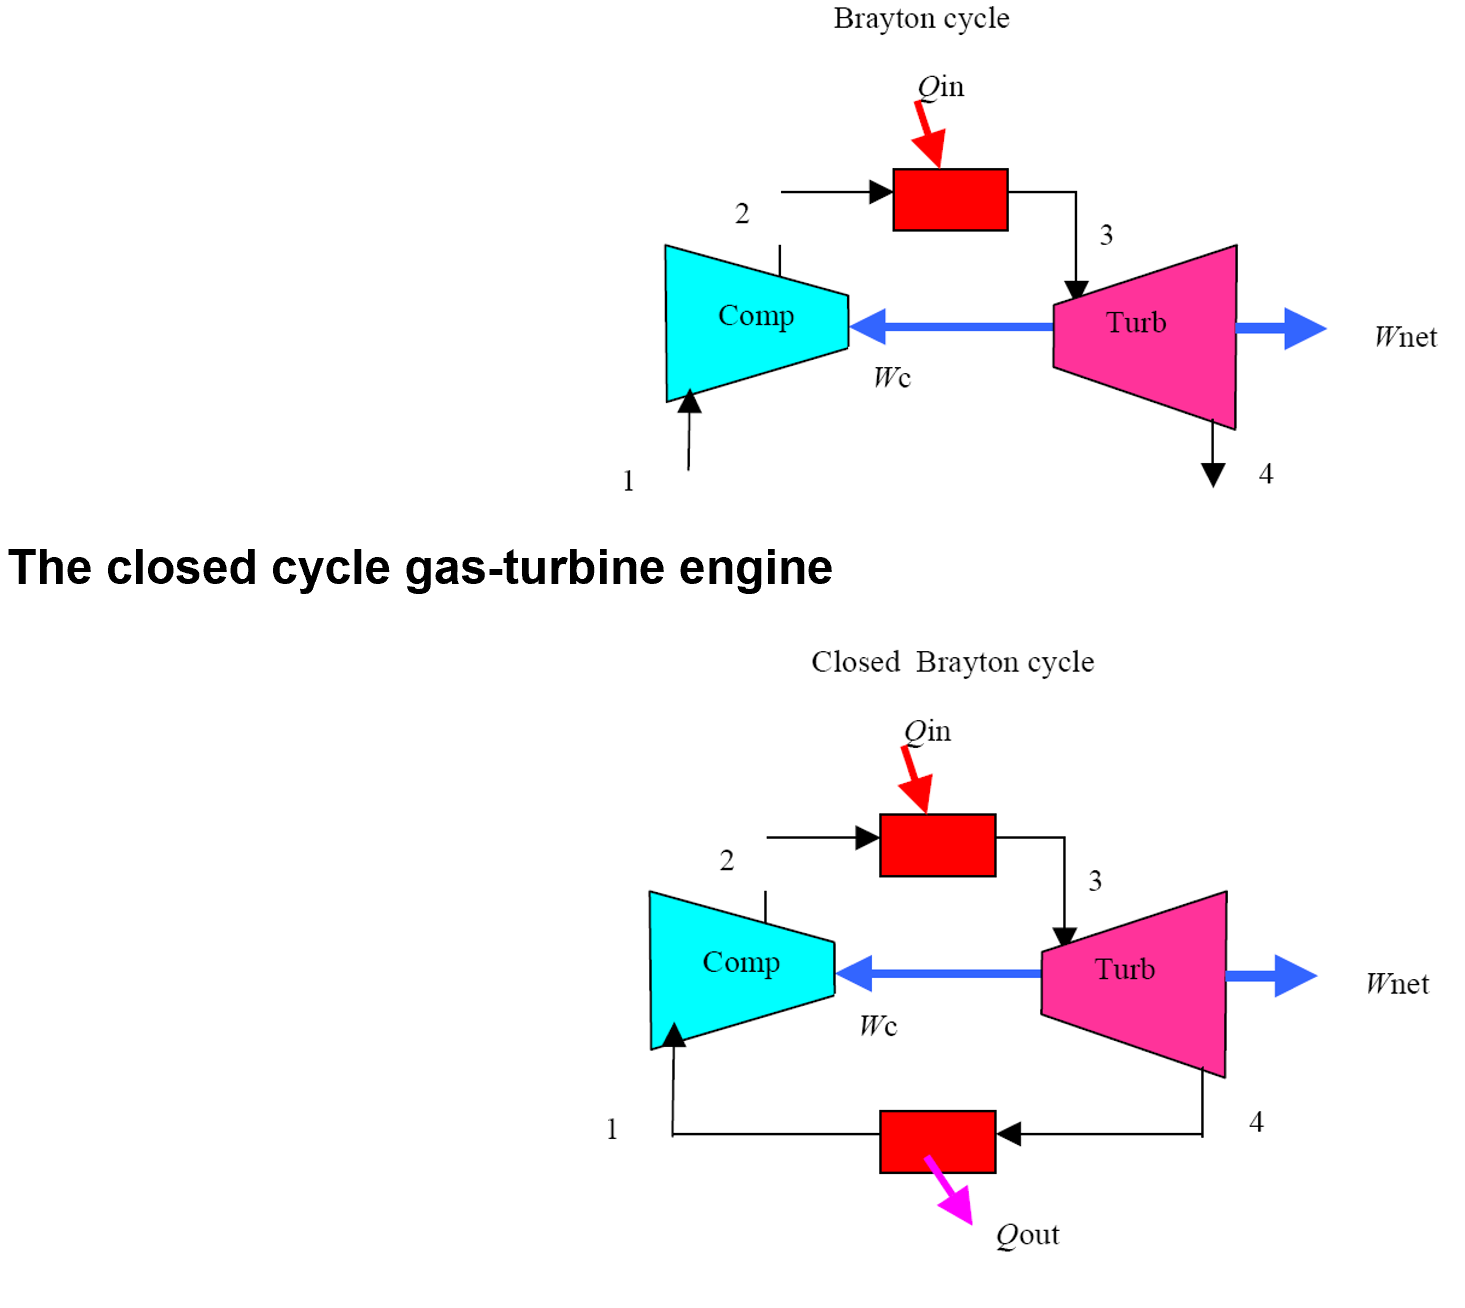
\includegraphics[width=\linewidth, height=5cm]{ClosedCycle_GasTurbineEngine.png}
\end{Figure}
\begin{Figure}
    \centering
    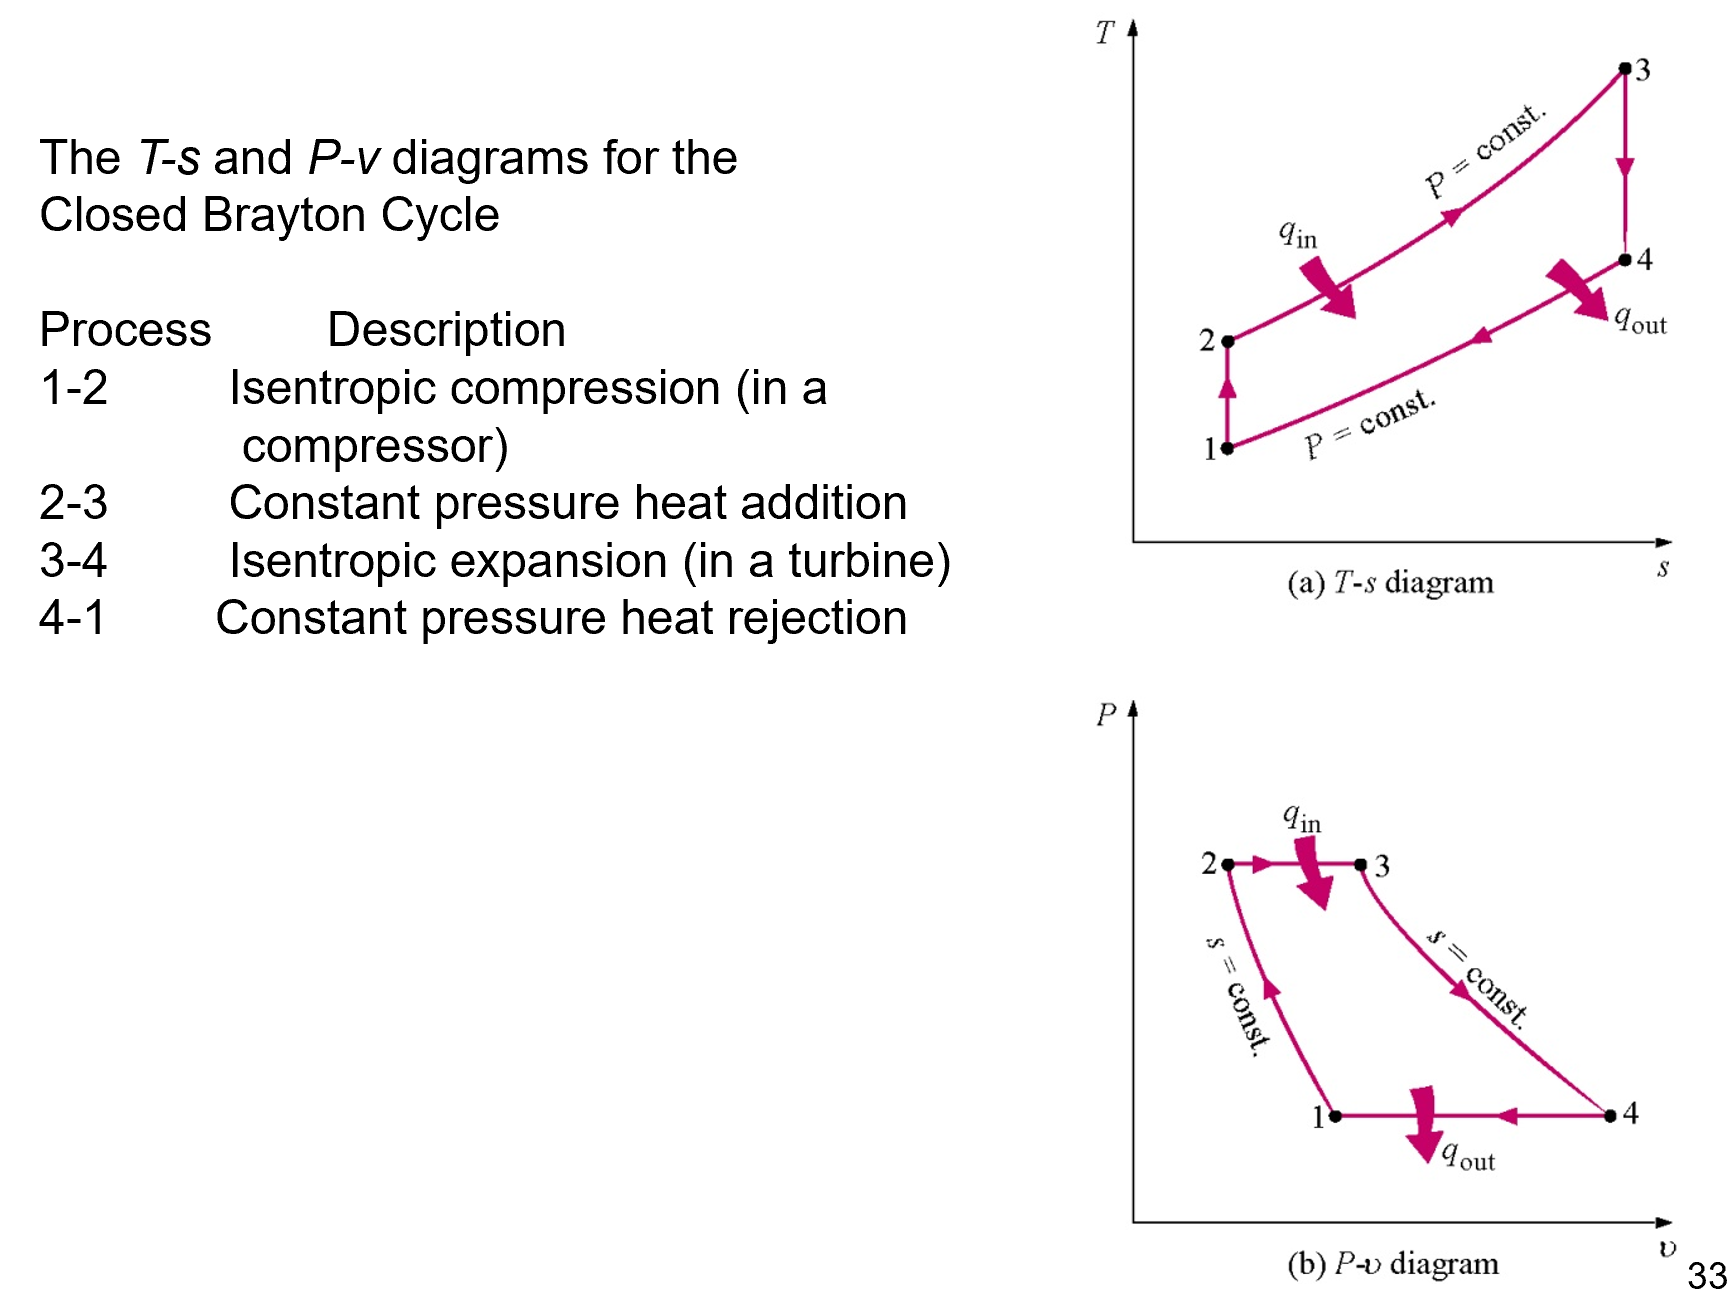
\includegraphics[width=\linewidth, height=5cm]{BraytonCycleClosed_PVTS.png}
\end{Figure}
\subsubsection{Pressure Ratio}
\begin{equation}
    r_p=\frac{P_2}{P_1}
\end{equation}
\begin{equation}
    \eta_{th,Brayton}=\frac{W_net}{q_{in}}=1-\frac{1}{r_p^{(k-1)/k}}
\end{equation}
\subsubsection{**Back Work Ratio**}
\begin{equation}
    BWR=\frac{w_in}{w_out}=\frac{w_comp}{w_turb}
\end{equation}
\subsubsection{General Brayton Cycle Equations}
\begin{equation}
    W_{\text{net, out}}=w_{\text{a,t,out}}-w_{\text{a,c,in}}=\nu_t-w_sT_{out}-\frac{w_{\text{s,c,in}}}{\nu_c}
\end{equation}
\begin{equation}
    w_{\text{s, net, out}}=w_{\text{s, t, out}}-w_{\text{s, c, in}}
\end{equation}

\subsection{Regenerative Brayton Cycle}
\begin{Figure}
    \centering
    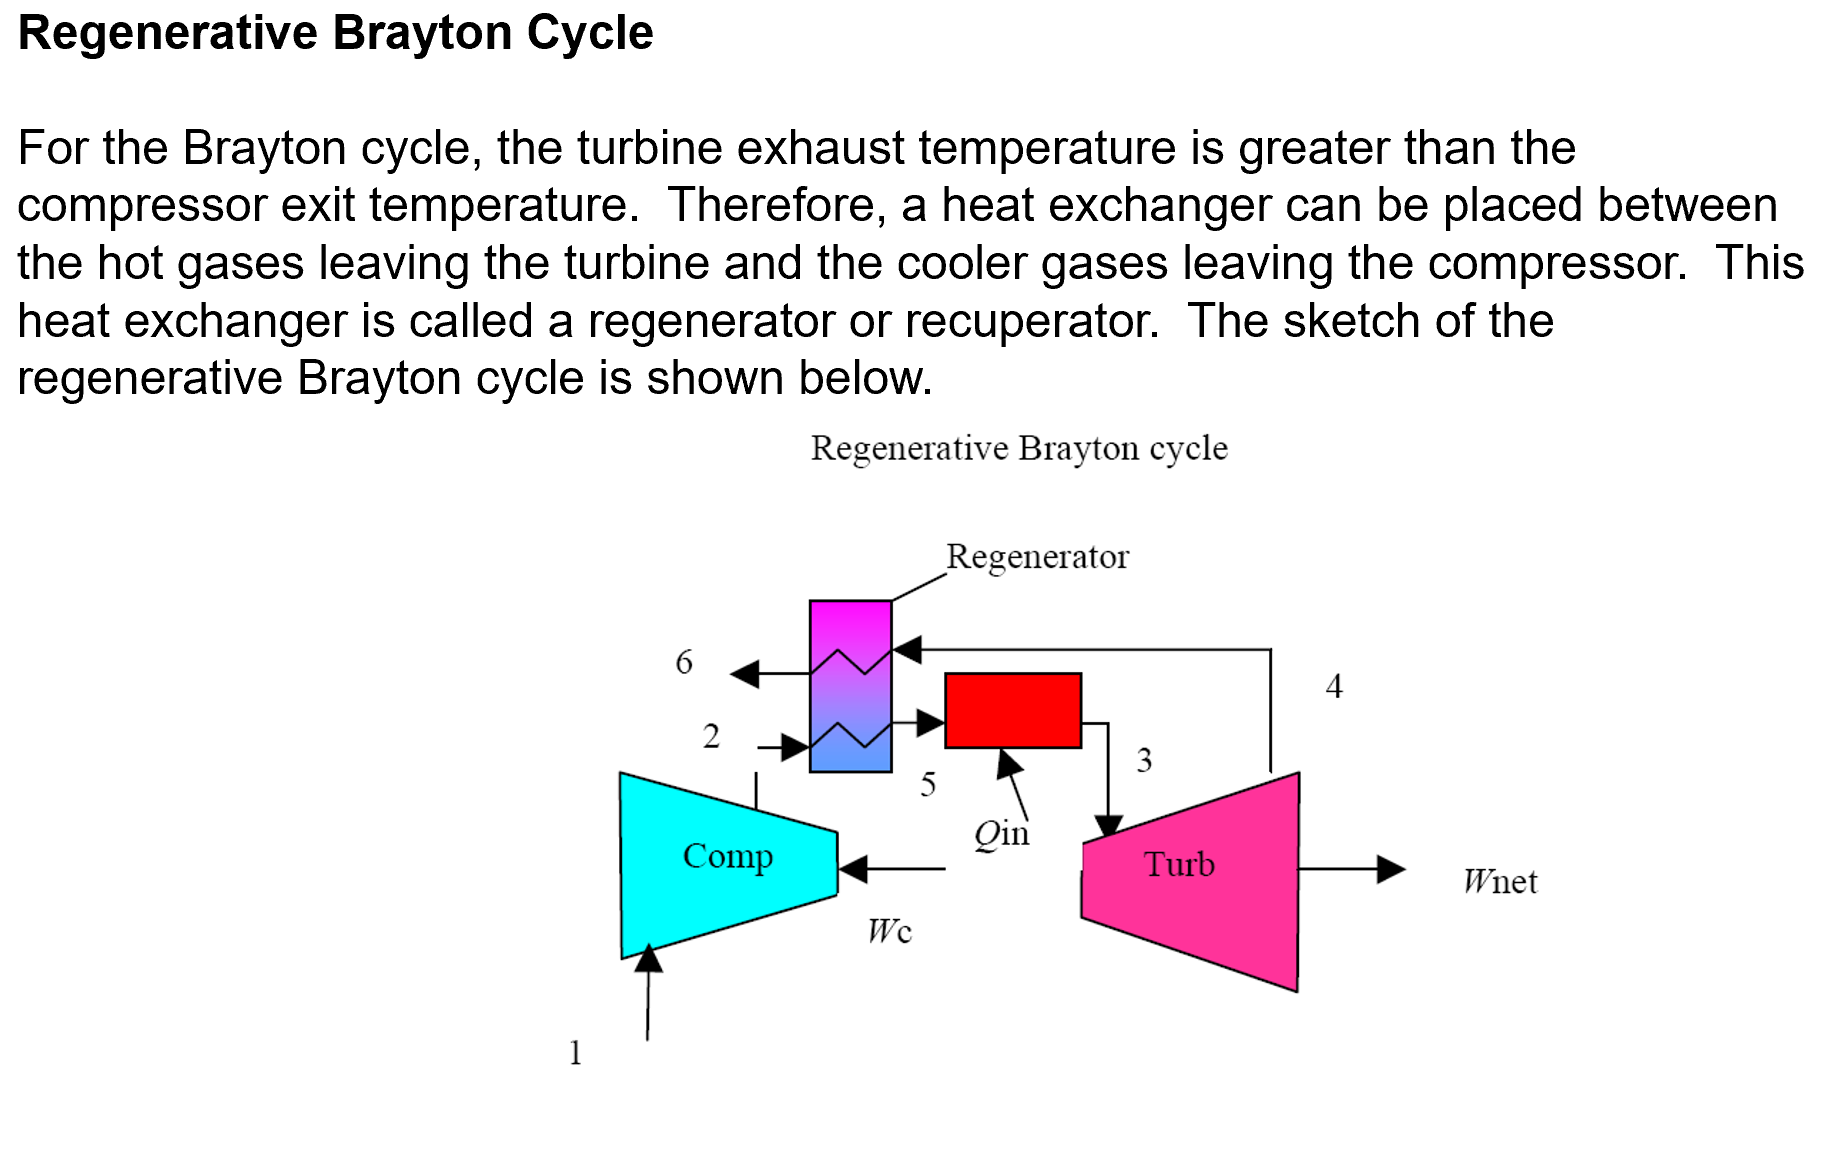
\includegraphics[width=\linewidth, height=5cm]{RegenerativeBrayton.png}
\end{Figure}
\begin{Figure}
    \centering
    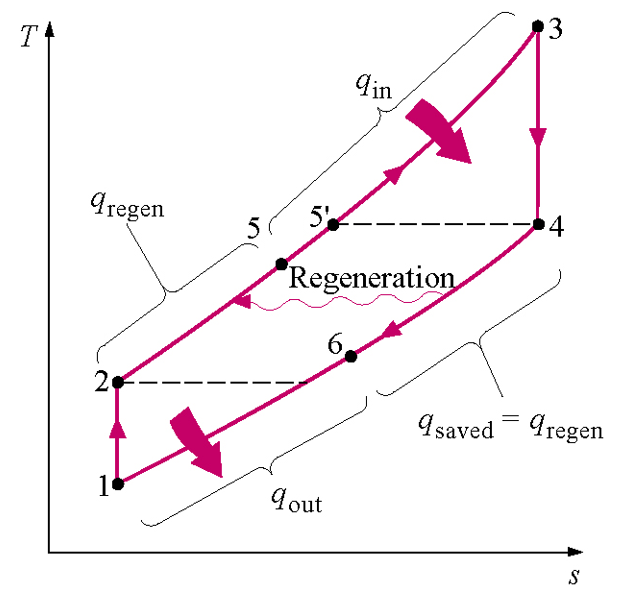
\includegraphics[width=\linewidth, height=5cm]{BraytonRegenerative_TS_Diagram.png}
\end{Figure}
\begin{equation}
    \sigma_{regen}=\frac{q_{regen,act}}{q_{regen,max}}=\frac{h_5-h_2}{h_4-h_2}
\end{equation}
\subsubsection{Thermal Efficiency}
\begin{equation}
    \eta_{th,regen}=1-\frac{q_{out}}{q_{in}}=1-\frac{h_6-h_1}{h_3-h_5}
\end{equation}

\section{Chapter 10}
\subsection{Rainkine Cycle}
\begin{Figure}
    \centering
    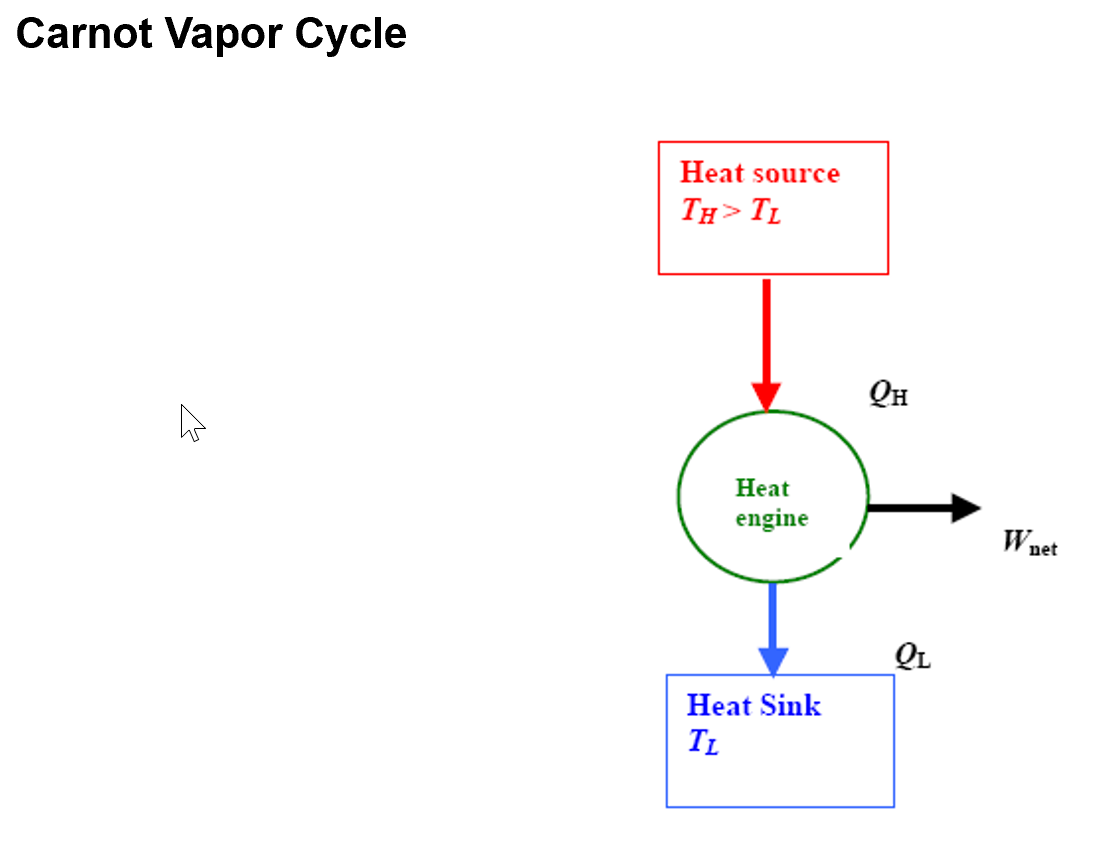
\includegraphics[width=\linewidth, height=5cm]{Carnot_VaporCycle.png}
\end{Figure}
\begin{Figure}
    \centering
    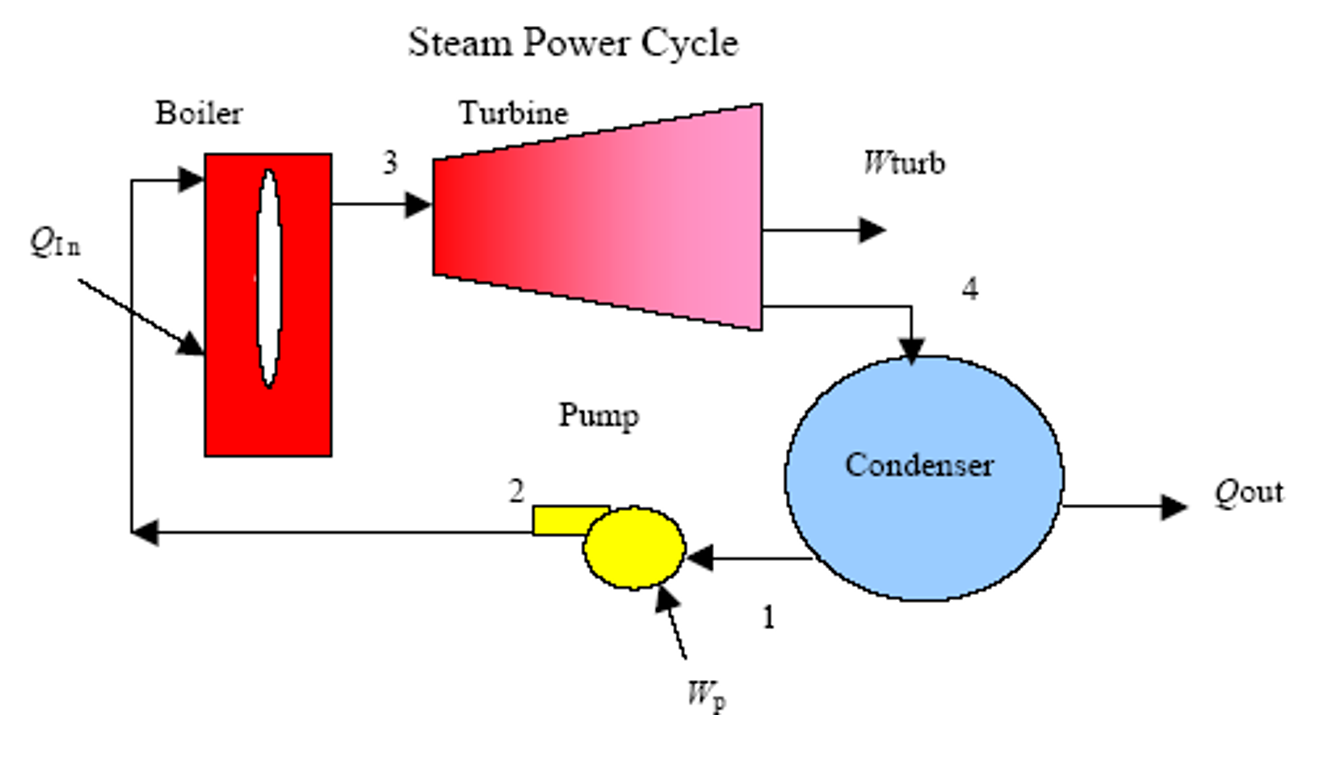
\includegraphics[width=\linewidth, height=5cm]{SteamPowerCycle.png}
\end{Figure}
\begin{Figure}
    \centering
    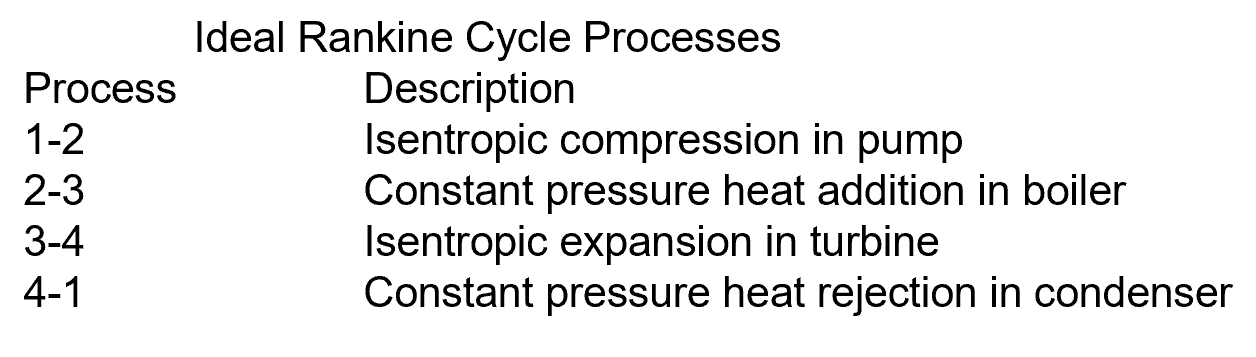
\includegraphics[width=\linewidth]{RankineCycleProcess.png}
\end{Figure}

\section{MSC}
\subsection{Isentropic Compression}
\begin{equation}
    v_{r2}=\frac{V_2}{v_1}v_{r1}=\frac{1}{r}v_{r1}
\end{equation}
\subsection{Isentropic Expansion}
\begin{equation}
    v_{r2}=\frac{V_2}{v_1}v_{r1}
\end{equation}
\subsection{General}
\begin{equation}
    \dot{m}_s=\frac{\dot{w}_{\text{net,out}}}{\dot{w}_{\text{s,net,out}}}=\frac{\text{kg}}{\text{s}}
\end{equation}
\begin{equation}
    \dot{m}=\frac{\dot{q}_{\text{in}}}{\text{Heat Value}}    
\end{equation}

\section{11 - Refrigeration Cycles}
\begin{equation}
    \text{COP}_R=\frac{\text{Desired output}}{\text{Required output}}=\frac{\text{Cooling Effect}}{\text{Work input}}=\frac{Q_l}{W_{\text{net, in}}}
\end{equation}
\begin{equation}
    \text{COP}_HP=\frac{\text{Desired output}}{\text{Required input}}=\frac{\text{Heating Effect}}{\text{Work input}}=\frac{Q_H}{W_{\text{net, in}}}
\end{equation}
\begin{equation}
    \text{COP}_{\text{R, Carnot}}=\frac{1}{T_h/T_L-1}
\end{equation}
\begin{equation}
    \text{COP}_{\text{HP, Carnot}}=\frac{1}{1-T_L/T_H}
\end{equation}
\begin{equation}
    \text{COP}_R=\frac{Q_l}{W_{\text{net, in}}}=\frac{q_L}{w_{\text{comp,in}}}-w_{\text{turb,out}}
\end{equation}
\begin{equation}
    \text{COP}_{\text{absorption}}=\frac{\text{Desired output}}{Required input}=\frac{Q_L}{q_{\text{gen}}+W_{\text{pump}}}\approxeq\frac{Q_L}{Q_{\text{gen}}}
\end{equation}
\begin{equation}
    \text{COP}_{\text{rev,absorption}}=\nu_{\text{th,rev}}\text{COP}_{\text{R,rev}}=(1-\frac{T_0}{T_s})(\frac{T_L}{T_0-T_L})
\end{equation}
%\subsection{1 Refrigerators and Heat Pumps}
%\subsection{2 The Reversed Carnot Cycle}
%\subsection{3 - The Ideal Vapor-Compression Refrigeration Cycle}
%\subsubsection{4 - Actual Vapor-Compression Refrigeration Cycle}
%\subsection{5 - Second-Law Analysis of Vapor-compression Refrigeration Cycle}
%\subsection{6 - Selecting the Reight Refrigerant}
%\subsection{7 - Heat Pump System}
%\subsection{8 - Innovative Vapor-Compression Refrigeration Systems}
%\subsection{9 - Gas Refrigeration Cycles}
%\subsection{10 - Absorption Refrigeration Systems}

\section{Chapter 12}

\section{Chapter 13}

\section{Chapter 14 - Gas-Vapor Mixtures and Air-Conditioning}
\subsection{1 - Dry and Atomspheric Air}
\subsection{2 - Specific and Relative Humidity of Air}
\subsection{Absolute or Specific Humidity (Humidity Ratio)}
Dry Air $\rightarrow$ $\omega$=0
\begin{equation}
    \omega=\frac{m_v}{m_a}=\text{kg water vapor/kg dry air}
\end{equation}
\subsubsection{Relative Humidity}
\begin{equation}
    \psi=\frac{m_v}{m_g}=\frac{P_v\vee/R_vT}{P_g\vee/R_VT}=\frac{P_v}{P_g}
\end{equation}
\subsection{3 - Dew-Point Temperature}




% References
%\rule{0.3\linewidth}{0.25pt}
%\scriptsize
%\bibliographystyle{abstract}
%\bibliography{Bibliography}

% End of document
\end{multicols}
\end{document}